\documentclass[11pt,a4paper]{article}
\usepackage[utf8]{inputenc}
\usepackage[T1]{fontenc}
\usepackage{lmodern}
\usepackage[british]{babel}
\usepackage[margin=2.4cm]{geometry}
\usepackage{amsmath}
\usepackage{booktabs}
\usepackage{tabularx}
\usepackage{graphicx}
\usepackage{caption}
\usepackage{enumitem}
\usepackage{makecell}
\usepackage{xcolor}
\usepackage[authoryear,round]{natbib}
\usepackage[colorlinks=true,linkcolor=blue!50!black,citecolor=blue!50!black,urlcolor=blue!50!black]{hyperref}

\captionsetup{font=small,labelfont=bf}
\setlist{itemsep=2pt,topsep=4pt}
\newcolumntype{L}{>{\raggedright\arraybackslash}X}
\renewcommand{\arraystretch}{1.15}

% Units and symbols
\newcommand{\Kpe}{K\,EgC$^{-1}$}
\newcommand{\Pgk}{PgC\,K$^{-1}$}
\newcommand{\Pgp}{PgC\,ppm$^{-1}$}
\newcommand{\bL}{$\beta_L$}
\newcommand{\gL}{$\gamma_L$}
\newcommand{\bO}{$\beta_O$}
\newcommand{\gO}{$\gamma_O$}
\newcommand{\etaN}{$\eta_N$}

\title{Testing process-flag interpretive models for CMIP:\\ a TCRE case study}
\author{B.\,M. Sanderson\\ \small CICERO Center for International Climate Research}
\date{16 October 2026}

\begin{document}
\maketitle

\section*{Summary}

We tested the process-flag interpretive models of \citet{marvel2026} against two criteria the paper states: decompose only to the level where evidence exists, and choose interpretive models for parsimony and accuracy. As a test case we used a development configuration that applies these models to TCRE; the TCRE assessment itself is not yet written, and the configuration's numbers are illustrative, not results anyone has reported.

Two findings concern the published methods. On the CMIP6 ensemble, process effects other than nitrogen are not identified by presence flags; the nitrogen effect is, and the configuration's nitrogen decomposition reproduces the end-to-end difference in TCRE between nitrogen-limited and other models. Synthetic tests show, however, that common calibration practices can mask or distort flag-estimated effects, so their physical meaning depends on how models were developed. Two findings concern the development configuration: its real-world estimate does not predict held-out models better than the raw ensemble, and it sits about 0.19\,\Kpe{} above the TCRE implied by the CMIP6 inputs, roughly half from the nitrogen effect and half from process terms set by priors. We suggest design choices for the TCRE application while it is still being developed.

\section*{Context and scope}

\paragraph{What is published.} \citet{marvel2026} set out interpretive models for CMIP evidence: random-effects and correlated random-effects models, a process model in which a binary flag records whether each ESM includes a process and a scaling factor (\etaN{} for nitrogen) is inferred from the difference between the flagged and unflagged groups (their \S3.5, with a multi-process generalisation in \S4.3), updates from paired process experiments (\S4.3), and hierarchical emergent constraints (\S4.2). The paper applies the process model to \bL{} and reports that \bL{} is revised downward once nitrogen limitation is accounted for.

\paragraph{What is in development.} A public development repository (\texttt{netzeroasap/TCRE\_Assessment}) applies these models to every term in
\begin{equation}
  \mathrm{TCRE} = \frac{\alpha}{k + \beta + \alpha\gamma},
\end{equation}
with a multiplicative process model for \bL, an additive one for \gL{} with an interannual-variability constraint on its tropical part, and a joint emergent constraint (AMOC, sea-surface salinity, chemical uptake capacity) for \bO{} and \gO. In this configuration the real-world value of each land term is its baseline with every process switched on at ensemble-average effect ($U \times \prod\eta + \sum\delta$). We ran it as found at one commit; it gives 1.77\,\Kpe{} (95\,\% HDI 0.90 to 2.71). Its priors, inputs and structural choices are provisional and may change, and nothing here describes a finished assessment.

\paragraph{What we ask.} We do not question the Bayesian framing or the value of making interpretive choices explicit. The question is whether flag-based process models, applied to about 13 CMIP6 models, extract information from the ensemble or mainly express their priors. The development configuration is used because it is a fuller application of the published methods than the paper's \bL{} example. Findings~1 and~2 bear on the published methods; findings~3 and~4 describe the development configuration.

\section{The process decomposition goes beyond the evidence}
\label{sec:ident}

Only the nitrogen effect is recovered from synthetic data; permafrost, fire and vegetation effects return their priors. We generated pseudo-ensembles on the real 13-model process table with known effects, refitted the additive process model for \gL{} from the development code with its priors, and repeated each case 12 times (Table~\ref{tab:ident}).

\begin{table}[ht]
\centering\small
\caption{Synthetic identifiability of the additive process model for \gL. Values are truth $\to$ mean posterior estimate in \Pgk.}
\label{tab:ident}
\begin{tabularx}{\textwidth}{Lcccc}
\toprule
Synthetic truth & $\delta$ nitrogen & $\delta$ permafrost & $\delta$ fire & $\delta$ veg \\
\midrule
S1: data follow the model's own structure & $10 \to 12.4$ & $-30 \to -36.4$ & $-5 \to -0.5$ & $5 \to 0.1$ \\
S2: no permafrost effect, a $\pm15$ offset on the three CLM-based models & $10 \to 13.2$ & \makecell{$0 \to -29.4$\\(90\,\% cov.\ 0)} & $-5 \to 0.4$ & $5 \to 0.3$ \\
S3: nitrogen acts on $\beta$ only, reaching $\gamma$ through the COU$-$BGC interaction & \makecell{$0 \to 8.5$\\(90\,\% cov.\ 0)} & $-30 \to -35.0$ & $-5 \to -0.4$ & $5 \to -0.1$ \\
\bottomrule
\end{tabularx}
\end{table}

\begin{itemize}
\item \textbf{Permafrost.} The estimate is about $-30$\,\Pgk, the prior median, whether the true effect is $-30$ or zero. The flag is set for exactly CESM2, NorESM2-LM and CMCC-ESM2, which share the CLM land model, so a family offset is indistinguishable from a permafrost effect. The negative-definite prior cannot cover a zero effect.
\item \textbf{Fire and vegetation.} Estimates shrink to zero with posterior sd equal to the prior sd (about 9 against 10\,\Pgk).
\item \textbf{Nitrogen.} Recovered when the data follow the model's structure. When the nitrogen effect acts on $\beta$ and reaches $\gamma$ only through the interaction term, it is attributed to a direct $\delta_N$ of $+8.5 \pm 5.4$ with zero coverage: separate $\eta$ (on $\beta$) and $\delta$ (on $\gamma$) parameters double-count a single mechanism.
\end{itemize}

Against the paper's own criterion (``decompose the model to the level where evidence exists''), three of the four land process terms are beyond the evidence in CMIP6 when identified through presence flags. In the development configuration their posteriors carry prior information through to TCRE without being updated by it.

\section{The nitrogen effect carries through to TCRE; its historical signature is not visible}
\label{sec:nitrogen}

Models with nitrogen limitation have a 27\,\% lower \bL{} than the rest and a 6\,\% higher carbon factor $R$, the direction a weaker land sink implies (Fig.~\ref{fig:nitrogen}). The development configuration's own nitrogen decomposition (\etaN{} on \bL, $\delta_N$ on \gL) reproduces this: it predicts a ratio of 1.075 (5--95\,\% 1.015 to 1.139) against the observed 1.063, with $\delta_N$ on \gL{} offsetting about 40\,\% of the \bL{} effect. The group difference in \bL{} from which the paper's process model infers \etaN{} (its \S3.5 and Fig.~3) is real (permutation $p \approx 0.05$, 6 against 5 models).

\begin{figure}[ht]
\centering
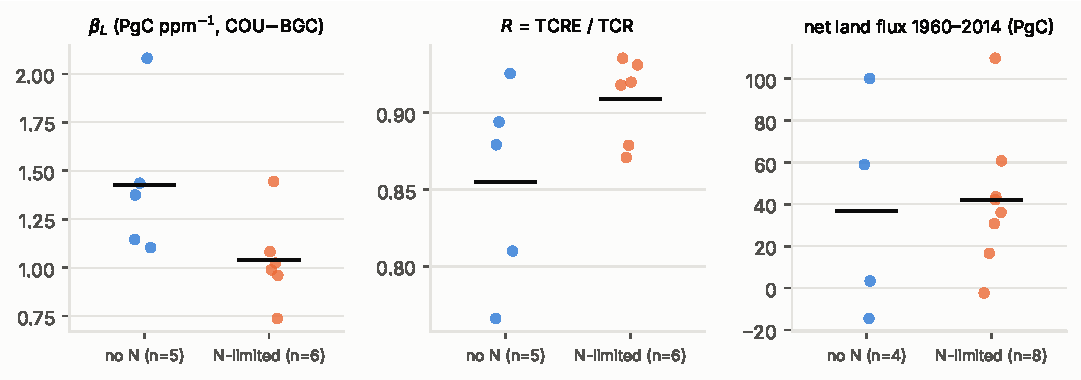
\includegraphics[width=\textwidth]{figures/nitrogen.pdf}
\caption{Nitrogen-limited and other models: \bL{} (COU$-$BGC convention) and $R$ from CMIP6 C4MIP 1pctCO2 (11 models), and 1960--2014 net land flux from historical runs. Horizontal bars are group means. Nitrogen flags from the process table in the development code. Source: \texttt{scripts/m7\_nitrogen\_historical.py}.}
\label{fig:nitrogen}
\end{figure}

The historical land sink is the weak leg. The nitrogen-limited models' 1960--2014 net land flux is not smaller (42 against 37\,PgC), where their \bL{} and \gL{} differences would imply about 15 to 25\,PgC less; differences in land-use emissions between models (sd about 37\,PgC) make this test inconclusive. With the paired-experiment $\nu$ evidence on \gL{} the predicted ratio is 1.098, still consistent. Nitrogen is therefore the one process term that CMIP6 both identifies and supports end to end; Section~\ref{sec:development} asks what it measures physically.

\section{The development configuration does not predict held-out models}
\label{sec:perfect}

When each of 9 models in turn plays the real world, the configuration's real-world estimate lies above its TCRE in every case, by 0.43\,\Kpe{} on average, and no configuration beats the raw ensemble (Fig.~\ref{fig:perfect}, Table~\ref{tab:crps}). The held-out model is removed from all training data and its own simulated observables replace the observations.

\begin{figure}[ht]
\centering
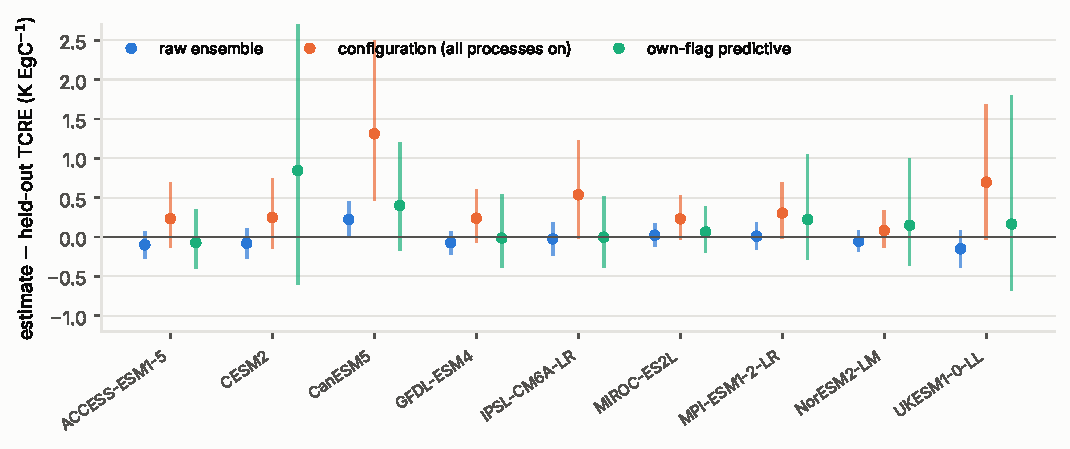
\includegraphics[width=\textwidth]{figures/perfect_model.pdf}
\caption{Leave-one-model-out errors in TCRE for 9 CMIP6 models: posterior mean minus the held-out model's value, with 5--95\,\% ranges (for the raw ensemble, mean $\pm 1.645$ sd). $\alpha$ is set to each model's own value. The own-flag interval for CESM2 extends beyond the axis. Source: \texttt{scripts/m4\_perfect\_model.py}.}
\label{fig:perfect}
\end{figure}

\begin{table}[ht]
\centering\small
\caption{Leave-one-model-out scores for TCRE.}
\label{tab:crps}
\begin{tabularx}{\textwidth}{Lccc}
\toprule
Leave-one-model-out & CRPS (\Kpe) & CRPS skill vs raw ensemble & 66\,\% / 90\,\% coverage \\
\midrule
Raw ensemble (training models' $R$ $\times$ own TCR) & 0.057 & 0 & 0.78 / 1.00 \\
Configuration estimate (all processes on) & 0.278 & $-3.9$ & 0.22 / 0.89 \\
Own-flag predictive & 0.111 & $-0.96$ & 0.89 / 1.00 \\
\bottomrule
\end{tabularx}
\end{table}

Leaving out whole model families gives the same result (skill $-3.6$ and $-0.84$). The offset of the configuration estimate is partly by design, since it adds process effects to every model; the point is that this adjustment is not tested by anything in CMIP. Using each model's own process flags removes most of the bias but gives intervals about four times wider than the ensemble, so the process regression adds spread without adding predictive information. By component, the land terms lose skill (\bL{} $-0.61$, \gL{} $-0.98$) and the ocean terms are near neutral (\bO{} $-0.05$, \gO{} $-0.10$). This is the test of accuracy that the paper names as a model-selection criterion in its \S3.6.

\section{In the development configuration, priors and structure set the shift}
\label{sec:priors}

The configuration's posterior lies 0.19\,\Kpe{} above the TCRE implied by the CMIP6 input means (1.74 against 1.55 at TCR 1.7\,K). Splitting the change in $k + \beta + \alpha\gamma$ by component, 86\,\% comes from the lower \bL, 36\,\% from the more negative \gL{} (process deltas, chiefly permafrost) and $-24$\,\% from a higher \bO. Within \bL, about 60\,\% of the reduction is the nitrogen factor ($\eta_N = 0.72$), which brings \bL{} to the mean of the nitrogen-limited models and is supported end to end (Section~\ref{sec:nitrogen}); about 40\,\% is the fire factor ($\eta_\mathrm{fire} = 0.86$), which this ensemble cannot identify. Roughly half of the shift therefore rests on CMIP evidence and half on terms set by priors (Table~\ref{tab:components}).

\begin{table}[ht]
\centering\small
\caption{Prior, posterior and CMIP6 input means for each carbon-cycle component in the development configuration.}
\label{tab:components}
\begin{tabularx}{\textwidth}{lcccL}
\toprule
Component & Prior median & Posterior mean & CMIP6 input mean & What moves it \\
\midrule
\bL{} (\Pgp) & 0.82 & 0.74 & 1.12 & $\eta$ factors applied to all models \\
\gL{} (\Pgk) & $-14$ & $-52$ & $-26$ & process $\delta$s, chiefly permafrost \\
\bO{} (\Pgp) & 1.01 & 1.00 & 0.90 & the prior on $\log\beta_O$; 1.16 with regression prior $\sigma = 1$ \\
\gO{} (\Pgk) & $-8.9$ & $-9.7$ & $-9.0$ & barely updated (KL 0.05) \\
\bottomrule
\end{tabularx}
\end{table}

As configured, the ocean component does not include the protection described in the paper's \S4.2, where a random-effects model pulls an emergent-constraint posterior back toward CMIP. Here the latent \bO{} has a fixed prior centred on 1.0, not a CMIP-informed one, and the posterior sits at that prior median, 1.4 CMIP standard deviations above the ensemble mean. Out of sample the constraint is neutral (CRPS skill $-0.05$ for \bO, $-0.10$ for \gO).

Single-prior changes move the TCRE mean from 1.67 (no permafrost effect) to 1.89 (wide $\eta$ priors) and the 95th percentile from 2.39 to 2.85. The structural-variance and LKJ priors change the mean by at most 0.02. The paper notes that the shared-bias fraction $\rho$ is prior-dominated (its Fig.~2b); in this configuration the same holds for the terms that set the central value.

\section{Comparison with the WCRP climate sensitivity assessment}
\label{sec:sherwood}

The WCRP assessment of climate sensitivity \citep{sherwood2020} avoids most of the problems found here, because it does not infer feedbacks from GCM ensemble statistics. It states that GCM sensitivity distributions are not independent of the historical record and that it avoids ``relying on GCMs to tell us what values to expect for key feedbacks except where the feedback mechanisms can be calibrated against other evidence'' (its \S1). Its process line is built from line-by-line radiative transfer, large-eddy simulation and observed variability, with GCMs used mainly as transfer functions. Table~\ref{tab:sherwood} sets the issues found here against its treatment.

\begin{table}[ht]
\centering\small
\caption{Issues found in the development configuration and their treatment in \citet{sherwood2020}. Section numbers refer to that paper.}
\label{tab:sherwood}
\begin{tabularx}{\textwidth}{>{\raggedright\arraybackslash}p{0.36\textwidth}L}
\toprule
Issue found in the development configuration & Treatment in \citet{sherwood2020} \\
\midrule
Process effects inferred from presence flags across about 13 models; three of four not identified & Each feedback component has a likelihood from process evidence outside the ensemble (\S3.2 to 3.4); a few cloud types rest mainly on expert judgement, stated as such with wide likelihoods \\
No end-to-end check of the decomposition & The summed feedback is checked against observed interannual radiation variability to catch missing feedbacks (\S3.5) \\
Models calibrated against the same evidence a process line would use (Section~\ref{sec:development}) & Identified as ``model selection bias'' (\S6.2) and the reason the ensemble is kept out of the process line \\
Prior influence not yet diagnosed & Prior predictive distributions and alternative priors reported; the upper tail's prior dependence is shown (\S7.2). The prior choices were later disputed \citep{lewis2022} \\
Emergent constraints used as primary evidence; neutral out of sample & Treated as a secondary, widened ``ad hoc'' likelihood, kept out of the baseline, with selection bias and dependence on the process line discussed (\S3.6) \\
Covariance between components discarded when combining & Feedbacks assumed additive and independent; GCM covariances set aside as not understood, with the effect on width discussed (\S3.4) \\
No analysis of dependence between land, ocean and TCR & Possible shared errors across lines examined; one reinforcing dependence (the pattern effect) found and quantified (\S6) \\
No out-of-sample test of accuracy & Also absent for the synthesis as a whole; the GCM-derived pattern-effect correction is the main shared exposure \\
$\beta$ and $\gamma$ depend on convention and forcing level & Target defined as an effective sensitivity over 150 years, with historical pattern and paleo state dependence modelled explicitly (\S4.2, \S5.2) \\
\bottomrule
\end{tabularx}
\end{table}

The ECS assessment therefore offers a template, and the development configuration departs from it at the points where our tests find problems. A TCRE synthesis on that template would take TCR from its own assessment, build the carbon factor from process evidence outside ESMs (free-air CO$_2$ enrichment and nutrient experiments for \bL{} and nitrogen limitation, observation-based ocean uptake, permafrost process studies), use ESMs as transfer functions, combine with the historical attribution line, and analyse dependence between lines. Process evidence for the carbon cycle is thinner than for clouds, so such a synthesis may be wider than the development configuration's posterior; its width would then reflect evidence rather than priors applied to the CMIP ensemble.

\section{Process effects, model development and static benchmarks}
\label{sec:development}

Flag-based estimates of process effects measure the development history of the models as much as their physics. No CMIP-scale ensemble can resolve most process effects, and in synthetic tests common development practices can push the one effect that is within reach, nitrogen on \bL, towards zero. In CMIP6 that effect survives (Section~\ref{sec:nitrogen}), but its physical meaning depends on how models were calibrated.

\paragraph{How large an ensemble?} A least-squares stand-in for the flag regression, with the scatter between models that the flags leave unexplained in the CMIP6 inputs (29\,\Pgk{} for \gL, 0.38 for $\log\beta_L$), gives the number of independent models needed for a two-standard-error detection (Table~\ref{tab:power}).

\begin{table}[ht]
\centering\small
\caption{Ensemble size needed to detect each process effect at two standard errors.}
\label{tab:power}
\begin{tabularx}{\textwidth}{Lccc}
\toprule
Effect & Standard error with 13 models & \makecell{Models needed,\\current flag mix} & \makecell{Models needed,\\balanced flags} \\
\midrule
Nitrogen on \bL{} ($-27$\,\%) & 0.28 in $\log\beta_L$ (effect 0.32) & about 50 & about 30 \\
Permafrost on \gL{} (30\,\Pgk) & 35 & about 80 & about 20 \\
Nitrogen on \gL{} (10\,\Pgk) & 21 & about 230 & about 140 \\
Fire or vegetation on \gL{} (5\,\Pgk) & 24 to 26 & 1,200 to 1,500 & about 530 \\
\bottomrule
\end{tabularx}
\end{table}

The models must be independent: CMIP6 has about a dozen distinct land carbon models, and extra versions of one land model add little. Design matters as much as size, since the permafrost flag is confined to CLM-based models and no number of further CLM models separates it from a CLM offset. Paired experiments within a model remove the scatter between models: two of them move $\delta_N$ from $18 \pm 10$ to $7 \pm 2$\,\Pgk, more than the whole ensemble does.

\paragraph{Calibration and recalibration.} Modelling groups report practices such as calibrating the productivity response to CO$_2$ against free-air CO$_2$ enrichment (FACE) experiments, aiming for good scores on aggregate benchmarks such as ILAMB, and recalibrating when a historical run's CO$_2$ or GPP is badly biased. We simulated these on the real nitrogen flags, with a true \etaN{} of 0.73: FACE calibration pulls each model part-way to the observed response; recalibration rescales turnover or allocation whenever the 1960--2014 land sink is more than 20\,PgC from target (Fig.~\ref{fig:devbias}).

\begin{figure}[ht]
\centering
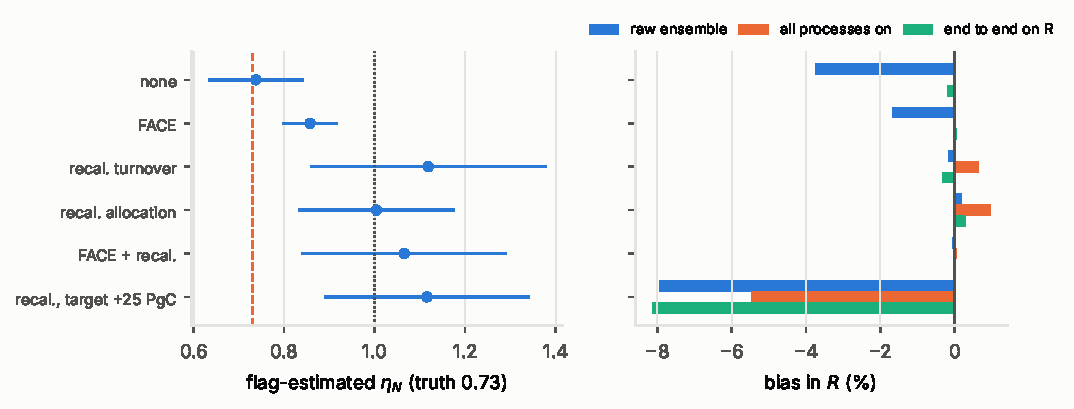
\includegraphics[width=\textwidth]{figures/development_bias.pdf}
\caption{Synthetic test of development practices. Left: flag-estimated \etaN{} (mean $\pm$ sd over replicates; dashed line the truth, 0.73; dotted line no effect). Right: bias in $R$ for three estimators. Recalibration tolerance 20\,PgC on the 1960--2014 land sink. Source: \texttt{scripts/m9\_tuning\_selection.py}.}
\label{fig:devbias}
\end{figure}

\begin{itemize}
\item \textbf{The process estimate is lost.} Under recalibration the flag regression returns \etaN{} of 1.00 to 1.12, that is no nitrogen effect; FACE calibration alone gives 0.86. The paper's Bayesian \bL{} model gives 1.03 and 0.98 in a check on a few replicates, against 0.79 with no development effects ($\hat r \le 1.006$, no divergences).
\item \textbf{The aggregate survives if the target is right.} Recalibration towards the true historical sink keeps $R$ within 1\,\% for every estimator, because development has already done the correcting.
\item \textbf{A wrong target is invisible.} Recalibration towards a sink 25\,PgC too high biases $R$ by $-5.5$\,\% (all processes on) to $-7.9$\,\% (raw ensemble). No flag analysis, perfect-model test or historical observable can detect this, because the whole ensemble is anchored to the same target.
\end{itemize}

\paragraph{Evidence from land-model development.}
\begin{itemize}
\item \emph{One flag spans very different behaviour.} CLM4 and CLM5 both carry the nitrogen flag, but CLM4 had strong nitrogen limitation and a CO$_2$ response below observations, while CLM5 responds more strongly to CO$_2$, a change evaluated against meta-analyses of FACE and nitrogen-addition experiments \citep{wieder2019}. Nitrogen-fixation flexibility, extraction costs and stoichiometric flexibility dominate the fertilisation response \citep{fisher2019}. A binary flag records that a process is coded, not how strongly it limits; across CMIP6, \etaN{} partly records how each group calibrated its nitrogen scheme.
\item \emph{Variation within one model rivals variation between models.} In a perturbed-parameter ensemble of CLM5.1, plausible parameter values change the response of net ecosystem production to raising CO$_2$ from 367 to 867\,ppm from about $+50$\,\% to a decrease \citep{kennedy2025}.
\item \emph{Static benchmarks do not constrain responses.} The parameters that set the present-day state are largely not those that control responses to CO$_2$, nitrogen or warming; triose phosphate limitation ranks 39th for present-day production but third for the high-CO$_2$ response \citep{kennedy2025}, and ``goodness of fit to present-day conditions does not necessarily imply a constraint on future transient projections'' \citep{fisher2019}. Calibration that acts on state parameters therefore neither compensates nor constrains the responses, which is consistent with the weak skill of present-day emergent constraints and historical observables found here.
\item \emph{Selection is built in.} Parameter ranges are commonly restricted so that all vegetation types survive pre-industrial and low-CO$_2$ conditions \citep{kennedy2025}, a filter on the response space that applies to CMIP models as well.
\end{itemize}

Comparisons across CMIP therefore compare differently calibrated codes, possibly calibrated against the same experimental evidence that a process line would use. Evidence that can identify process effects is of other kinds: perturbed-parameter ensembles within models, paired process switches across structurally different land models, and manipulation experiments used as response benchmarks \citep{wieder2019}, counted as independent only where models were not calibrated against them. That requires calibration metadata for each model alongside its process flags.

\medskip\noindent\emph{Disclosure: B.\,M. Sanderson is a co-author of \citet{fisher2019} and \citet{kennedy2025}.}

\section{Overall assessment}
\label{sec:assessment}

The Bayesian framing is sound and the nitrogen term is supported by CMIP6, but the rest of the process layer is set by priors, the process-adjusted estimate fails out of sample, and even the nitrogen term's physical meaning depends on model development that is only partly documented (Table~\ref{tab:findings}).

\begin{table}[ht]
\centering\small
\caption{Findings, their dependence on knowledge of model tuning, and confidence.}
\label{tab:findings}
\begin{tabularx}{\textwidth}{L>{\raggedright\arraybackslash}p{0.3\textwidth}>{\raggedright\arraybackslash}p{0.14\textwidth}}
\toprule
Finding & Depends on knowing how models were tuned? & Confidence \\
\midrule
Permafrost, fire and vegetation effects are not identified by presence flags (Sections~\ref{sec:ident}, \ref{sec:development}) & No: holds in synthetic data with no development effects & High \\
The nitrogen effect is identified and reproduces the end-to-end difference in $R$ (Section~\ref{sec:nitrogen}) & No for the statistical result; yes for its physical meaning & Medium (6 against 5 models) \\
About half of the configuration's shift rests on terms set by priors: the fire factor, permafrost and the \bO{} prior (Section~\ref{sec:priors}) & No & High \\
The ``all processes on'' estimate does not predict held-out models, and no configuration beats the raw ensemble (Section~\ref{sec:perfect}) & No & High \\
The ocean emergent constraint is neutral out of sample and \gO{} is prior-dominated (Section~\ref{sec:priors}) & No & Medium \\
Calibration against FACE or after biased historical runs can push flag-estimated \etaN{} towards 1 (Section~\ref{sec:development}) & Yes: the size depends on practices that are only partly known & Medium (synthetic) \\
A shared bias in calibration targets biases every estimator alike and cannot be detected within CMIP (Section~\ref{sec:development}) & Yes & Medium (synthetic) \\
\bottomrule
\end{tabularx}
\end{table}

\paragraph{What the nitrogen result means.} The CMIP6 nitrogen signal survives whatever calibration was done: lower \bL, less negative \gL{} and a higher $R$ in the nitrogen-limited models. Whether it is the physical effect of nitrogen limitation, or partly reflects how nitrogen-enabled models were calibrated (for example against FACE responses), cannot be decided without calibration metadata; the synthetic tests show that either is possible. Applying it to models without nitrogen limitation is justified to the extent that it is physical.

\paragraph{Reasoning with incomplete information on tuning.}
\begin{itemize}
\item Report process-adjusted estimates across a range of development scenarios (none, FACE calibration, recalibration after historical runs) rather than under one implicit assumption.
\item Collect calibration metadata from modelling groups (targets such as FACE responses, benchmark scores, historical CO$_2$ or GPP; whether recalibration followed historical runs) and code it alongside the process flags.
\item Discount experimental evidence that models may have been calibrated against, rather than counting it as independent of the ensemble.
\item Treat the ensemble as already calibrated to the historical record. A shared error in that target, and processes no model represents, need independent lines of evidence.
\end{itemize}

\paragraph{Verdict.} As a language for stating how CMIP relates to the real world, the approach is sound. As a way to infer process adjustments to TCRE from flags on CMIP6, it supports one term (nitrogen, with uncertain physical meaning) and otherwise expresses its priors. A defensible configuration would report the CMIP-consistent estimate (random effects, with the covariance between TCR and the carbon terms kept), the nitrogen adjustment with its evidence and caveats, and any further adjustment, such as for permafrost, as an explicit judgement coordinated with the remaining-carbon-budget term for unrepresented feedbacks. The largest uncertainty, TCR, and any shared bias lie outside what this machinery can resolve; independent lines (TCR $\times$ $R$, historical attribution, process evidence from outside ESMs) are needed for those.

\section*{Implications and suggestions}

The TCRE application is still being designed, so these are suggestions for its design, not corrections to a reported result. The limits we find are informational, not Bayesian: about 13 related models with binary process flags cannot identify process effects at this granularity. Three features of the interpretive model follow from that and would remain under any choice of priors.

\begin{enumerate}
\item \textbf{Identification.} Process effects other than nitrogen are asserted through priors, not learned from CMIP. The result is CMIP plus elicited adjustments, which is legitimate but should be presented and assessed as such.
\item \textbf{Target.} ``Every process on, at ensemble-average effect'' is an assumption that no CMIP-based test can check, and the 1960--2014 observables we examined (ocean sink, net land flux, airborne fraction of fossil emissions) do not discriminate the carbon factor across models.
\item \textbf{Coordinates.} $\beta$ and $\gamma$ depend on the COU$-$BGC convention and on forcing level ($2\times$ parameters underpredict $4\times$ TCRE by 11\,\%). For nitrogen the separate effects on $\beta$ and $\gamma$ partly cancel (Section~\ref{sec:nitrogen}); judging process effects end to end, on $R$, is the direct test.
\end{enumerate}

What we suggest:
\begin{itemize}
\item Place process adjustments on the carbon factor $R = \mathrm{TCRE}/\mathrm{TCR}$, or on the airborne fraction, where paired experiments can test them end to end.
\item Report a CMIP-consistent estimate beside the process-adjusted one, so the adjustment is visible and can be assessed on its own evidence.
\item Report prior-against-posterior diagnostics for each component and the TCRE sensitivity to the permafrost, $\eta$ and ocean-regression priors.
\item Adopt leave-one-model-out and leave-one-family-out tests as a standard check of accuracy, the criterion the paper names in its \S3.6. Our harness can be shared.
\item Use the paired-experiment $\gamma$ evidence already computed in the code ($\nu_N$, $\nu_\mathrm{fire}$, $\nu_\mathrm{veg}$). It moves $\delta_N$ from $18 \pm 10$ to $7 \pm 2$ and $\delta_\mathrm{fire}$ from $1 \pm 13$ to $-11 \pm 5$\,\Pgk.
\item Keep the cross-model covariance between TCR and the carbon terms; with it the 95th percentile falls from 2.58 to 2.35\,\Kpe.
\item Coordinate any permafrost adjustment with the remaining-carbon-budget term for unrepresented feedbacks, so it is not counted twice.
\end{itemize}

We agree with the paper that apparently strong relationships need not constrain the target: our own convention-free line (TCR $\times$ $R$) finds no historical observable with out-of-sample skill for $R$.

\section*{Methods, reproducibility and caveats}

\begin{itemize}
\item \textbf{Code and data.} Development code at a single commit (98c74cb), with internal variable names prefixed so the land models build (priors, likelihoods and structure unchanged); inputs from the project spreadsheet as of 2026-10-13. Every number here comes from a script with a fixed seed in the private repository \texttt{benmsanderson/tcre\_mini} (\texttt{results/SUMMARY.md} lists them); the figures are drawn by \texttt{scripts/note\_figures.py} from the saved results.
\item \textbf{Diagnostics.} $\beta$, $\gamma$ and $R$ from C4MIP 1pctCO2 BGC, COU and RAD global means (11 CMIP6 models, years 61 to 80, piControl linear drift removed). Historical observables from CMIP6 \texttt{historical} runs, 1960 to 2014; observational counterparts from the Global Carbon Budget 2025.
\item \textbf{Sampling.} PyMC 5.28, 4 chains $\times$ 1000 draws, \texttt{target\_accept} 0.99. All fits reported have $\hat r \le 1.01$; one divergence in 36 synthetic fits and none in the perfect-model fits.
\item \textbf{Perfect-model setup.} The held-out model (or family) is removed from all training data and from the paired nitrogen experiments; its own $\gamma_\mathrm{IAV}$, AMOC, SSS and CUC replace the observations with the real observational uncertainties. $\alpha$ is the held-out model's own value in both the development configuration and the baselines, so only the carbon-cycle part is tested.
\item \textbf{Caveats.} Ensembles are small (9 to 13 models); the nitrogen group comparison rests on 6 against 5 models (permutation $p \approx 0.05$ for \bL). The historical land flux includes land-use emissions that differ between models. The family table for leave-one-family-out is approximate. The development configuration is a snapshot: its priors, inputs and structure may have changed since, and it is not a finished assessment. The ``all processes on'' target may be a deliberate choice; our point is that its consequences are set by priors and are not tested.
\end{itemize}

\bibliographystyle{plainnat}
\bibliography{references}

\end{document}
